56. \begin{figure}[ht!]
\center{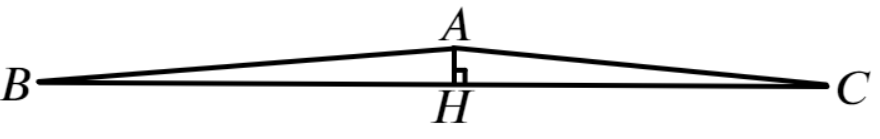
\includegraphics[scale=0.35]{g9-56.png}}
\end{figure}\\
Рассмотрим равнобедренный треугольник $ABC,$ у которого $AB=AC=2$м, а высота $AH=0,00001$м. Тогда по неравенству треугольника $BC<AB+AC=4$м, а площадь $S=\cfrac{1}{2}AH\cdot BC<\cfrac{1}{2}\cdot0,00001\cdot4=0,00002\text{ м}^2.$ Значит, такой треугольник существует.\\
